\exercise{Binary Polar PAM signal generation and matched filter decoding}

\paragraph{Explanation:}
For section a), I simply followed the given instructions. I created a
function called \mttext{get\_signals} that returns the PAM samples.
Later, I also included the matched filter output, which I achieved by
generating a constant array with \mttext{ones} and convolving it with
\mttext{conv}. A key point here is that I added a parameter,
\mttext{idxs}, to select which samples to extract from $r[n]$. This
parameter can accept a number, an array, or even nothing.
Additionally, I created a helper function,
\mttext{get\_rectangular\_modulation\_pulse}, to retrieve the pulse, as
the name suggests.
For section b), I implemented the \mttext{plot\_signal} function,
which allows you to plot the signal. Eventually, I extended the
function by adding an optional parameter to specify which axes the plot should
appear on. I also included an optional boolean flag to control
whether or not to show the samples that are multiples of $T$.
Finally, for section d), I built a GUI. As mentioned in the class
forum, I used the MATLAB App Designer, but I did it programmatically.
I also decided to implement it as a MATLAB class since I was curious
to explore object-oriented programming in MATLAB. The App Designer
syntax was new to me, so I relied heavily on online documentation.
One useful reference can be found
\href{https://www.mathworks.com/help/matlab/creating_guis/add-ui-components-to-app-designer-programmatically.html}{here}.
A key property I found useful in most UI elements was
\mttext{ValueChangedFcn}, which enabled me to define a callback
function and update values easily. Here's a list of features I implemented:
\begin{itemize}
\item Inputs: all the existing inputs I implemented in the
\mttext{get\_signals} function.
\begin{itemize}
\item All inputs, except for the samples, are implemented through a
    text input. The samples input uses a scroll bar.
\end{itemize}
\item A checkbox to toggle the visibility of the markers
\item Two plots to display each signal
\item A title displaying the course name, my name, and the date
\item A few additional details:
\begin{itemize}
\item The samples scroll bar is set to the default value of $N*Q$
\item When changing $N$ or $Q$, the scroll bar limits are updated accordingly
\item The GUI is responsive when resized
\end{itemize}
\end{itemize}
To create this, I used the following functions:
\begin{itemize}
\item \mttext{uifigure} for the GUI itself
\item \mttext{uilabel} for text labels
\item \mttext{uieditfield} for input fields
\item \mttext{uicheckbox} for the checkbox
\item \mttext{uiaxes} for the plot axes within the GUI
\item \mttext{uislider} for the slider
\end{itemize}

\paragraph{MATLAB Code:}

\textbf{Signal Generation}

\begin{tiny}
\verbatiminput{code/get_signals.m}
\end{tiny}

\textbf{Signal Plotting}

\begin{tiny}
\verbatiminput{code/plot_signal.m}
\end{tiny}

\textbf{GUI}

\begin{tiny}
\verbatiminput{code/gui.m}
\end{tiny}

\paragraph{Results:}

\begin{figure}[H]
\centering
\begin{minipage}{.5\textwidth}
\centering
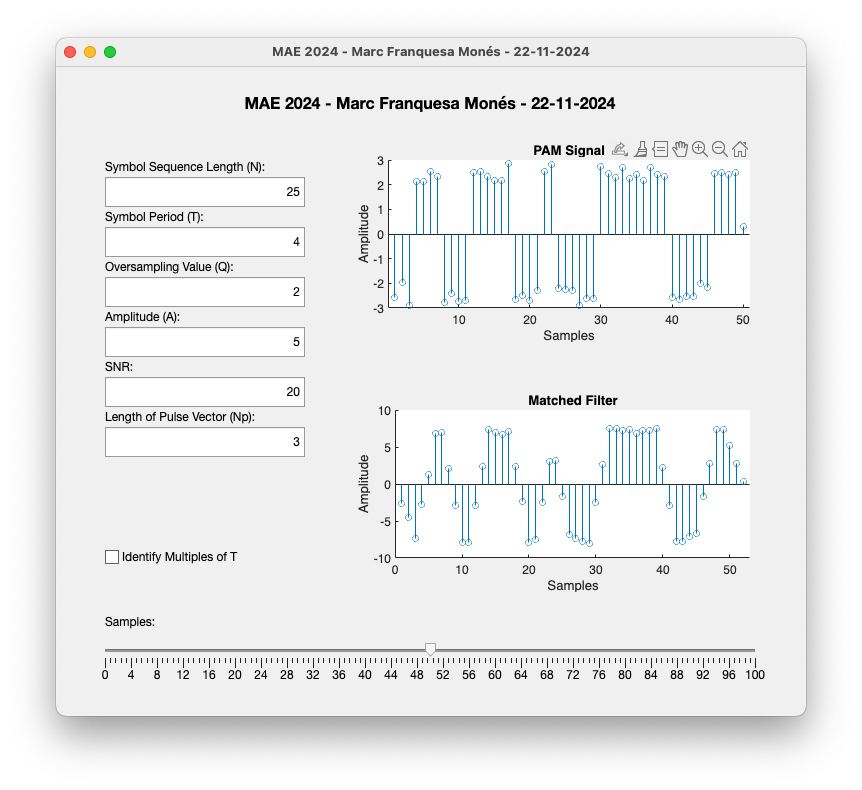
\includegraphics[width=\linewidth]{figures/1.png}
\caption{Default Values}
\label{fig:figures/1.png}
\end{minipage}%
\begin{minipage}{.5\textwidth}
\centering
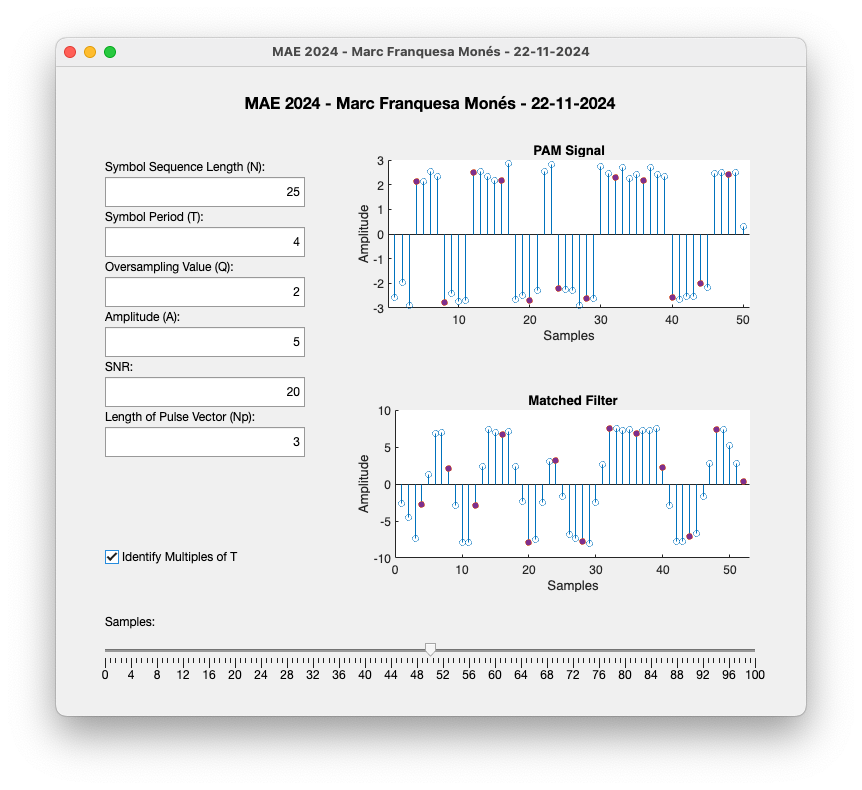
\includegraphics[width=\linewidth]{figures/2.png}
\caption{Marked $ T $ multiples}
\label{fig:figures/2.png}
\end{minipage}
\end{figure}

\begin{figure}[H]
\centering
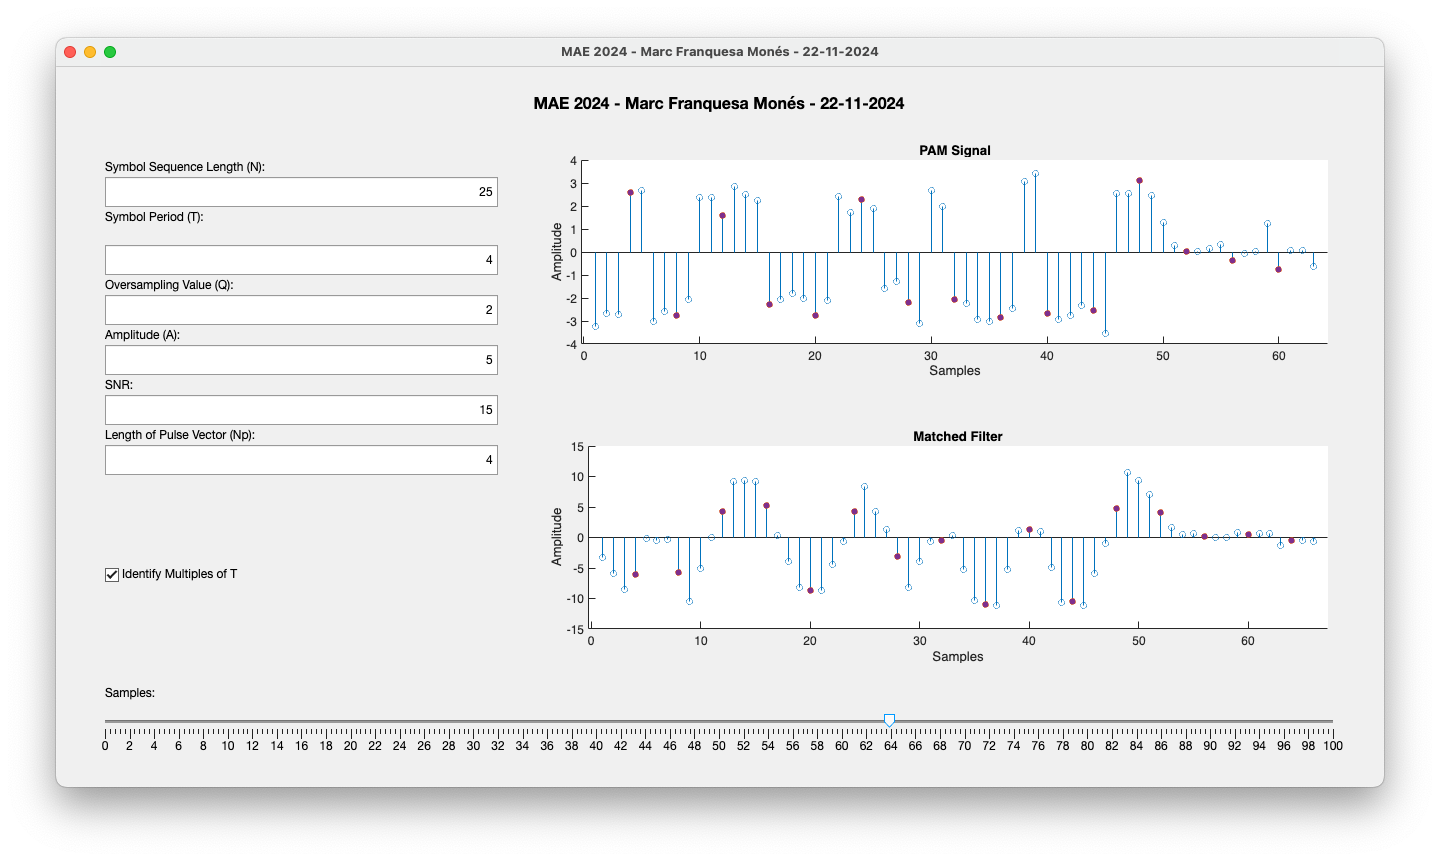
\includegraphics[width=10cm]{figures/3.png}
\caption{Resized and changed input parameters}
\label{fig:figures/3.png}
\end{figure}

Regarding how changing the parameters affects the result, some
observations are that:

\begin{itemize}
\item $ A $ affects the mean absolute value of the signal
\item Increasing $ SNR $ decreases PAM variance
\item A bigger $ N_p $ makes the matched filter output more uniform
\item If we increase the samples after $ N * Q $ we see that values
go to 0, we see the noise
\end{itemize}

\paragraph{Comments:}

I found creating the GUI in MATLAB pretty straightforward, you are
limited as to what you can do, but the things that are there work pretty well.
The main struggle I found was positioning everything in a decent way,
as, at least with how I implemented it, I have fixed $ x,y $ positions.

\bigskip
\hrule
